\part{GOAP}
\frame{\partpage}

\begin{frame}{GOAP}
    \begin{itemize}
        \pause\item \textbf{G}oal \textbf{O}riented \textbf{A}ction \textbf{P}lanning
        \pause\item Originally developed for F.E.A.R.\ (2005), since used in several games
        \pause\item A modified version of STRIPS specifically for real-time planning in video games
    \end{itemize}
\end{frame}

\begin{frame}{GOAP}
    \begin{itemize}
        \pause\item Each agent has a \textbf{goal set}
            \begin{itemize}
                \pause\item Multiple goals with differing \textbf{priority}
                \pause\item Goals are like in STRIPS --- sets of predicates that the agent wants to satisfy
            \end{itemize}
        \pause\item Each agent also has a set of \textbf{actions}
            \begin{itemize}
                \pause\item Like in STRIPS --- actions have preconditions and postconditions
                \pause\item Unlike STRIPS, each action also has a \textbf{cost}
            \end{itemize}
    \end{itemize}
\end{frame}

\begin{frame}{Action sets}
    \begin{itemize}
        \pause\item Different types of agent could have the \textbf{same goals} but \textbf{different action sets}
        \pause\item This will result in those agents achieving those goals in \textbf{different ways}
        \pause\item NB this doesn't have to be explicitly coded --- it \textbf{emerges} from the GOAP system
        \pause\item E.g.\ this was used by the F.E.A.R.\ team to quickly add new enemy types
    \end{itemize}
\end{frame}

\begin{frame}{Action sets}
    \begin{center}
        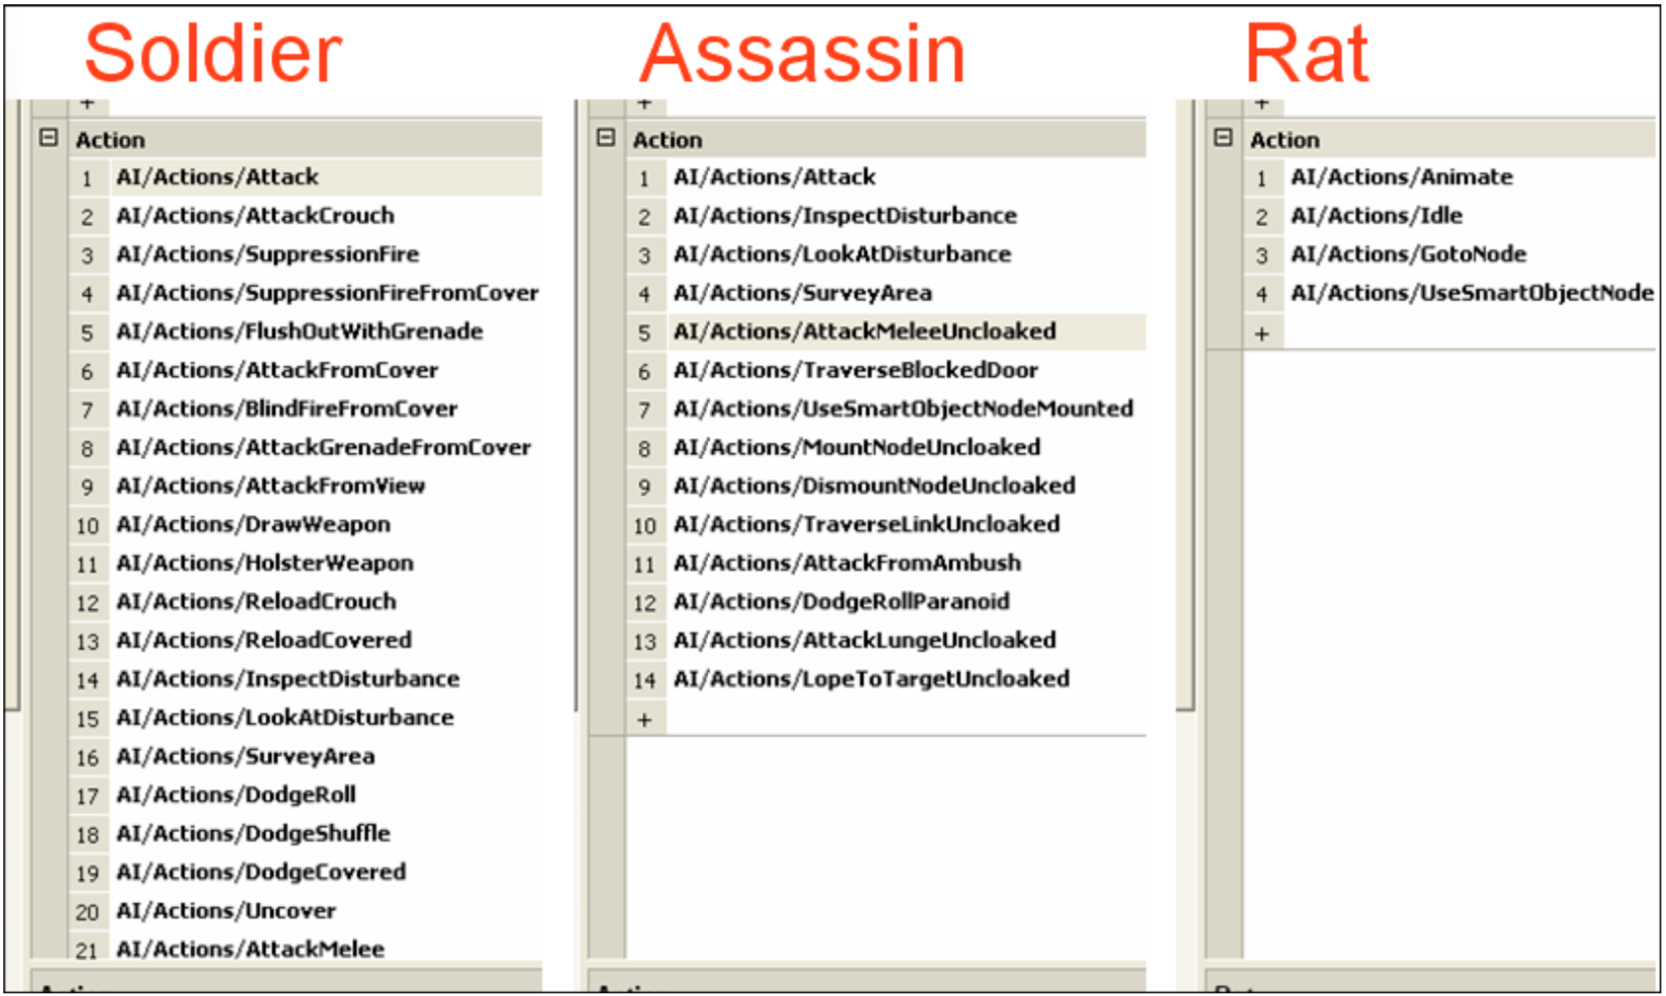
\includegraphics[width=\textwidth]{goap_action_sets}
    \end{center}
\end{frame}

\begin{frame}{Layering}
    \begin{itemize}
        \pause\item Goal set allows different behaviours with different priorities to be \textbf{layered}
        \pause\item E.g.\ enemy AI in F.E.A.R.:
    \end{itemize}
    \begin{center}
        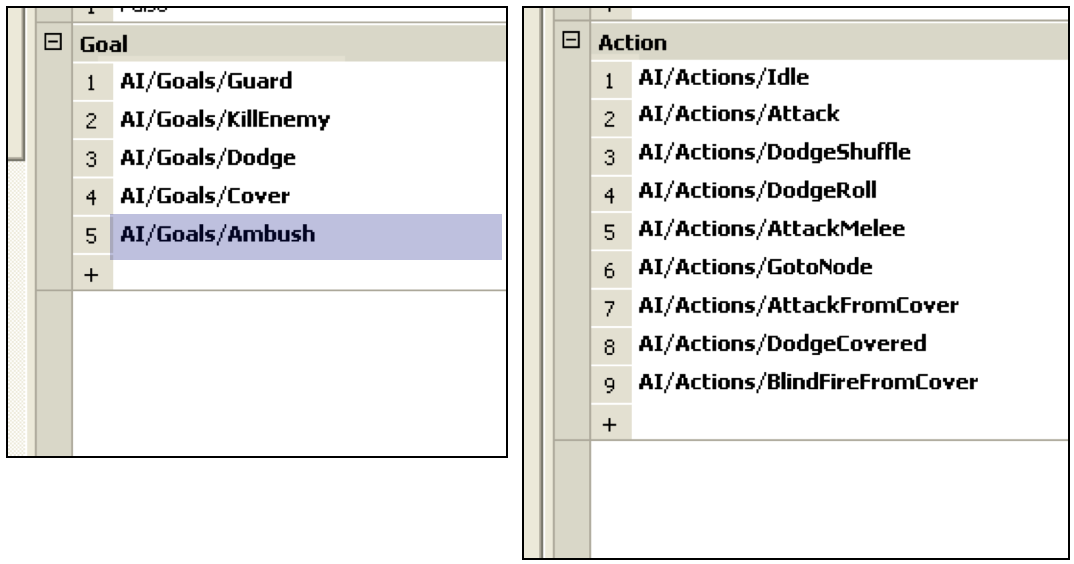
\includegraphics[width=0.8\textwidth]{goap_layering}
    \end{center}
\end{frame}

\begin{frame}{Implementing GOAP}
    \begin{itemize}
        \pause\item An \textbf{abstracted} view of the game world is used for planning
        \pause\item Represented as a fixed-length array (or struct) of values
        \pause\item Predicates (preconditions, postconditions, goals)
            represented in terms of this array representation
        \pause\item Most implementations also allow for \textbf{programmatic} preconditions
            (e.g.\ calling the pathfinding system to check availability of a path)
    \end{itemize}
\end{frame}

\begin{frame}{Implementing GOAP}
    \begin{itemize}
        \pause\item Not difficult to implement
        \pause\item Open-source implementations do exist
        \pause\item Not built into Unity or Unreal, but asset store packages are available
    \end{itemize}
\end{frame}

\begin{frame}{Finding the plan}
    \begin{itemize}
        \pause\item As in STRIPS, we can build a \textbf{state-action graph}
        \pause\item Since actions have costs, we can use \textbf{Dijkstra's algorithm} to find the lowest cost path to the goal
        \pause\item (or A* if we can find a suitable heuristic)
        \pause\item Plan is a \textbf{queue} of actions that the agent then executes
        \pause\item If the plan is interrupted or fails then the agent can \textbf{replan}
    \end{itemize}
\end{frame}

\begin{frame}{Using GOAP}
    \begin{itemize}
        \pause\item Planning is suitable when achieving a goal requires a specific \textbf{sequence of actions}
        \pause\item Especially when the plan is not obvious, or when you want to let the plan be \textbf{emergent}
        \pause\item Does require \textbf{abstraction} in a real-time videogame setting, though STRIPS-like definitions give a useful framework for this
    \end{itemize}
\end{frame}

\begin{frame}{``AAA game AI'' compared:\\GOAP vs behaviour trees}
    \begin{itemize}
        \pause\item BT: Designer specifies ``how''
        \pause\item GOAP: Designer specifies ``what'' --- ``how'' is in whatever system is used to implement
            actions (FSMs in F.E.A.R.; could use BTs or hand coding)
        \pause\item Both: actions (tasks in BT) are modular and reusable between agents
        \pause\item GOAP: goals are also modular and reusable
        \pause\item BT: goals are not represented explicitly
        \pause\item BT can be classified as \textbf{authored behaviour}
        \pause\item GOAP can be classified as \textbf{computational intelligence}
    \end{itemize}
\end{frame}

